\chapter{Технологическая часть}

\section{Средства реализации}

Для решения поставленной задачи была выбрана СУБД $PostrgeSQL$, так как она поддерживает такие функции, как связность таблиц, транзакционность, поддержка сложных структур, таких как \textit{json}, а так же имеется опыт работы с данной системой управления базами данных~\cite{postgres}.

В качестве языка программирования для серверной части был выбран язык \textit{С\#}~\cite{csharp}, так как в стандартной библиотеке языка присутствует поддержка всех структур данных, выбранных по результатам проектирования.

В качестве среды разработки была выбрана среда $Rider$, так как у него есть встроенный отладчик, а так же можно применять изменения в режиме реального времени.

Для реализации взаимодействия с базой данный используется фреймворк \textit{Entity Framework}~\cite{entity}, который обеспечивает сопоставление отношений объектов. Так же поддерживает он запросы $LINQ$, отслеживание изменений, обновления и миграции схемы.


\section{Создание таблиц}

В части работы \ref{sec:сущности} были описаны таблицы базы данных, соответствующий код для создания этих таблиц приведен в листинге \ref{lst:table1}--\ref{lst:table3}.

\begin{center}
	\captionsetup{justification=raggedright,singlelinecheck=off}
	\begin{lstlisting}[label=lst:table1,caption={Код на SQL для создания таблицы Users}]
CREATE TABLE IF NOT EXISTS "Users" (
	id UUID PRIMARY KEY,
	role INT NOT NULL,
	email VARCHAR(100) NOT NULL,
	password VARCHAR(100) NOT NULL
);
	\end{lstlisting}
\end{center}
\clearpage

\begin{center}
	\captionsetup{justification=raggedright,singlelinecheck=off}
	\begin{lstlisting}[label=lst:table2,caption={Код на SQL для создания таблиц Trainers, Admins, Workouts, Memberships, Schedules}]
CREATE TABLE IF NOT EXISTS "Trainers" (
	id UUID PRIMARY KEY NOT NULL REFERENCES "Users" (id),
	name VARCHAR(50) NOT NULL,
	gender VARCHAR(10) NOT NULL CHECK (gender IN ('male', 'female')),
	specialization VARCHAR(50) NOT NULL,
	experience INT NOT NULL,
	rating INT NOT NULL CHECK (rating >= 1 AND rating <= 5)
);

CREATE TABLE IF NOT EXISTS "Admins" (
	id UUID NOT NULL REFERENCES "Users" (id),
	name VARCHAR(50) NOT NULL,
	date_of_birth DATE NOT NULL, 
	gender VARCHAR(10) NOT NULL CHECK (gender IN ('male', 'female'))
);

CREATE TABLE IF NOT EXISTS "Workouts" (
	id UUID PRIMARY KEY,
	name VARCHAR(50) NOT NULL,
	description VARCHAR(200) NOT NULL,
	trainer_id UUID NOT NULL REFERENCES "Trainers" (id),
	duration INTERVAL NOT NULL,
	level INT NOT NULL CHECK (level >= 1 AND level <= 5)
);
CREATE TABLE IF NOT EXISTS "Memberships" (
	id UUID PRIMARY KEY,
	name VARCHAR(50) NOT NULL,
	duration INTERVAL NOT NULL,
	price INT NOT NULL,
	freezing INT NOT NULL
);

CREATE TABLE IF NOT EXISTS "Schedules" (
	id UUID PRIMARY KEY,
	workout_id UUID NOT NULL REFERENCES "Workouts" (id),
	date_and_time TIMESTAMP NOT NULL,
	client_id UUID REFERENCES "Clients" (id)
);
	\end{lstlisting}
\end{center}

\begin{center}
	\captionsetup{justification=raggedright,singlelinecheck=off}
	\begin{lstlisting}[label=lst:table3,caption={Код на SQL для создания таблиц Clients, Products, ClientProducts, Bonuses}]
CREATE TABLE IF NOT EXISTS "Clients" (
	id UUID PRIMARY KEY NOT NULL REFERENCES "Users" (id),
	name VARCHAR(50) NOT NULL,
	gender VARCHAR(10) NOT NULL CHECK (gender IN ('male', 'female')),
	date_of_birth DATE NOT NULL,
	membership_id UUID NOT NULL REFERENCES "Memberships" (id),
	membership_end DATE NOT NULL,
	remain_freezing INT,
	freezing_intervals json
);

CREATE TABLE IF NOT EXISTS "Products" (
	id UUID PRIMARY KEY,
	type VARCHAR(50) NOT NULL,
	name VARCHAR(50) NOT NULL,
	price INT NOT NULL
);

CREATE TABLE IF NOT EXISTS "ClientProducts" (
	id UUID PRIMARY KEY,
	id_client UUID NOT NULL REFERENCES "Clients" (id),
	id_product UUID NOT NULL REFERENCES "Products" (id)
);

CREATE TABLE IF NOT EXISTS "Bonuses" (
	id UUID PRIMARY KEY,
	client_id UUID NOT NULL REFERENCES "Clients" (id),
	count INT NOT NULL
);
	\end{lstlisting}
\end{center}


\section{Создание ролей на уровне базы данных}

По спроектированным в части работы \ref{sec:роли} ролям базы данных, были созданы роли на уровне базы данных, соответствующих код представлен в листинге~\ref{lst:roles}.

\begin{center}
	\captionsetup{justification=raggedright,singlelinecheck=off}
	\begin{lstlisting}[label=lst:roles,caption={Код на SQL для создания ролей}]
CREATE ROLE guest;
GRANT SELECT ON TABLE public."Products", public."Memberships", public."Schedules", public."Trainers", public."Workouts" TO guest;

CREATE ROLE client;
GRANT SELECT ON TABLE public."Bonuses", public."Products", public."Memberships", public."Schedules", public."Trainers", public."Workouts" TO client;
GRANT INSERT ON TABLE public."Schedules" TO client;
GRANT UPDATE ON TABLE public."Clients" TO client;

CREATE ROLE trainer;
GRANT SELECT ON TABLE public."Schedules", public."Clients", public."Workouts" TO trainer;
GRANT INSERT, UPDATE, DELETE ON TABLE public."Schedules", public."Workouts" TO trainer;
GRANT UPDATE ON TABLE public."Trainers" TO trainer;

CREATE ROLE admin;
GRANT ALL PRIVILEGES ON ALL TABLES IN SCHEMA public TO admin;
	\end{lstlisting}
\end{center}

\section{Создание триггера}

Код для создания триггера и соответствующей функции, алгоритм которой был в части работы \ref{sec:триггер}, представлен с листинге~\ref{lst:trigger}.

\clearpage
\begin{center}
	\captionsetup{justification=raggedright,singlelinecheck=off}
	\begin{lstlisting}[label=lst:trigger,caption={Код на SQL для создания триггера и функции}]
CREATE OR REPLACE FUNCTION update_bonus_count()
RETURNS TRIGGER AS $$
DECLARE
	product RECORD;
	total_cost NUMERIC;
	available_bonus_count INTEGER;
	bonus_payment INTEGER;
	max_bonus_count INTEGER;
	product_type VARCHAR(100);
BEGIN
	SELECT price INTO total_cost FROM public."Products" WHERE id = NEW.id_product;
	SELECT count INTO available_bonus_count 
	FROM public."Bonuses" 
	WHERE client_id = NEW.id_client;
	IF NEW.write_off THEN
	SELECT (total_cost * 0.5) 
	INTO max_bonus_count;
	bonus_payment := LEAST(available_bonus_count, max_bonus_count);
	total_cost := total_cost - bonus_payment;
	available_bonus_count := available_bonus_count - bonus_payment;
	END IF;
	available_bonus_count := available_bonus_count + (total_cost * 0.1);
	SELECT type INTO product_type FROM public."Products" WHERE id = NEW.id_product;
	IF product_type = 'PersonalWorkout' THEN
	available_bonus_count := available_bonus_count + 100;
	END IF;

	UPDATE public."Bonuses" SET count = available_bonus_count WHERE client_id = NEW.id_client;
	
	RETURN NULL
END;
$$ LANGUAGE plpgsql;
CREATE TRIGGER on_client_product_insert
AFTER INSERT ON public."ClientProducts"
FOR EACH ROW
EXECUTE FUNCTION update_bonus_count();
	\end{lstlisting}
\end{center}

\section{Тестирование}

Проводилось тестирование функции, алгоритм которой приведен в части работы~\ref{sec:триггер}. 

Были составлены следующие классы эквивалентности:
\begin{enumerate}[label=\arabic*)]
	\item у клиента нет бонусов;
	\item у клиента бонусов менее половины стоимости
	товара;
	\item спроектировать сущности базы данных и ограничения целостности фитнес-клуба;
	\item количество бонусов клиента равно половине
	стоимости товара;
	\item у клиента бонусов более половины стоимости
	товара;
	\item клиент покупает персональную тренировку.
\end{enumerate}

Каждый тестовый случай анализировался со включенным списанием бонусов и без него.


\section{Примеры веб-интерфейса программы}

На рисунках \ref{fig:pr1} и \ref{fig:pr2} представлен интерфейс, который видит пользователь при входе на сайт.


\begin{figure}[h!]
	\centering
	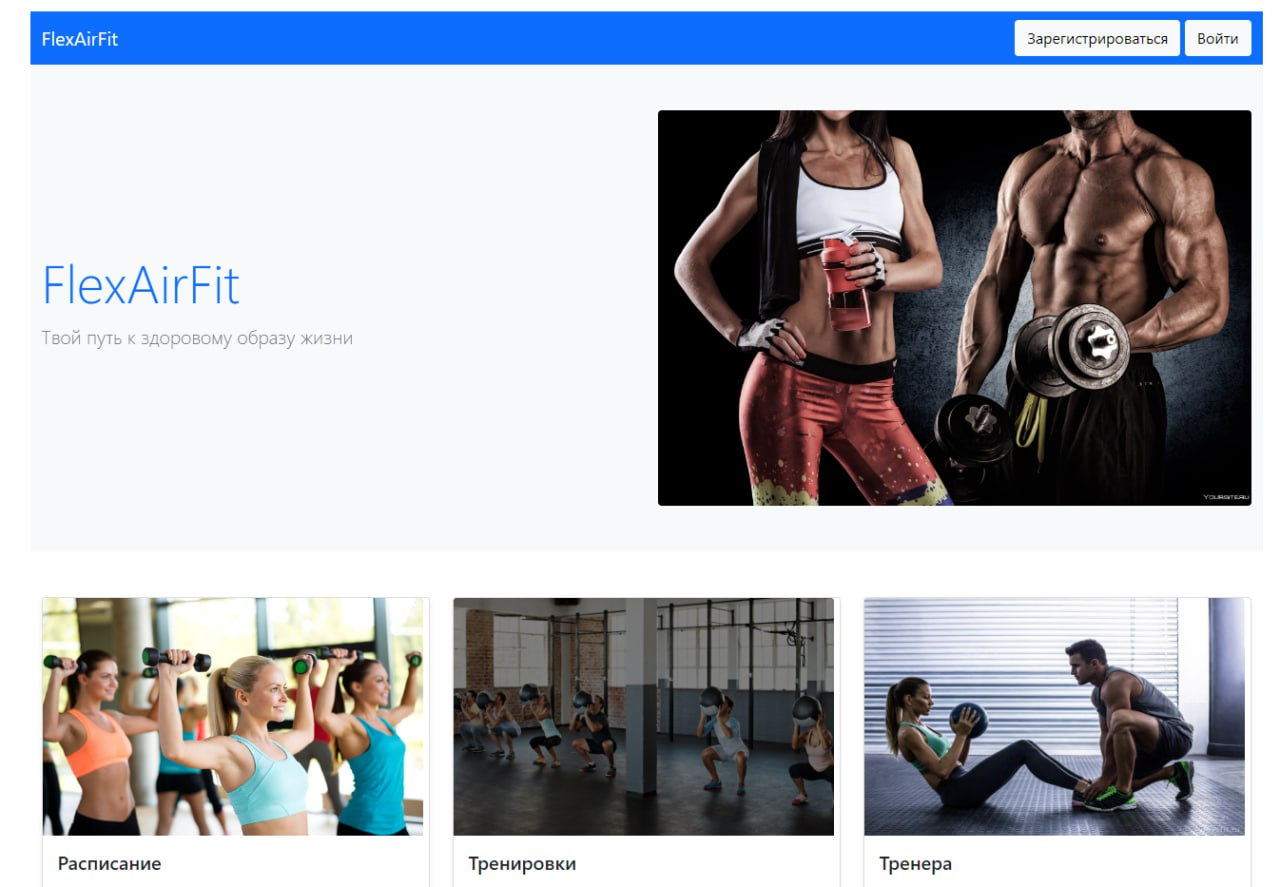
\includegraphics[width=\linewidth]{img/pr1}
	\caption{Пример интерфейса}
	\label{fig:pr1}
\end{figure}

\begin{figure}[h!]
	\centering
	
\includegraphics[width=\linewidth]{img/pr2}
	\caption{Пример интерфейса}
	\label{fig:pr2}
\end{figure}
\clearpage

\section{Выводы к технологической части}

В данной части были рассмотрены средства реализации, разработано программное обеспечение, рассмотрен интерфейс и тестирование.